
\section{Mécanismes de l'hypersensibilité aux très faibles doses de rayonnement}

L'hypersensibilité aux très faibles doses (HRS, \textit{Hyper-Radiosensitivity}) est un phénomène 
dans lequel une cellule présente une réponse biologique disproportionnée pour des doses 
inférieures à environ $0.3$--$0.5\ \mathrm{Gy}$. Elle est généralement suivie d'une zone de 
\textit{radio-résistance induite} (IRR). Les mécanismes principaux pouvant expliquer ce comportement
sont détaillés ci-dessous.

\subsection{Activation insuffisante de la réparation de l'ADN}

À très faibles doses, le nombre de cassures double brin (DSB) est faible, mais inférieur au seuil 
nécessaire pour déclencher une activation complète des voies de réparation. Les protéines clés 
comme ATM, ATR, DNA-PKcs ou Rad51 ne sont recrutées qu'à un niveau suboptimal.

\begin{itemize}
    \item Activation partielle d'ATM/ATR.
    \item Formation inefficace de foyers $\gamma$-H2AX.
    \item Recrutement incomplet des voies NHEJ et HR.
\end{itemize}

Ainsi, même un faible nombre de lésions demeure mal réparé, entraînant une létalité plus élevée 
qu'attendue.

\subsection{Absence d'activation des checkpoints du cycle cellulaire}

Les faibles niveaux de dommages ne permettent pas d'activer pleinement les contrôles du cycle cellulaire 
(Chk1/Chk2), entraînant :

\begin{itemize}
    \item absence d'arrêt en G2/M ;
    \item poursuite de la réplication sur un ADN endommagé ;
    \item augmentation de la mort mitotique.
\end{itemize}

\subsection{Vulnérabilité de cibles subcellulaires critiques}

Même quelques événements ionisants peuvent affecter des structures hautement sensibles, telles que :

\begin{itemize}
    \item les centrosomes ;
    \item les fourches de réplication ;
    \item les mitochondries (création secondaire de ROS).
\end{itemize}

Ces dommages, touchant des cibles essentielles, amplifient la réponse cellulaire.

\subsection{Effets intercellulaires : l’effet bystander}

Les cellules irradiées émettent des signaux (ROS, NO, cytokines) modifiant la réponse de cellules voisines.  
Ainsi, une dose très faible appliquée localement peut provoquer une réponse non linéaire et amplifiée.

\subsection{Transition HRS $\rightarrow$ IRR}

Dès que la dose dépasse un seuil (souvent $\sim 0.5\ \mathrm{Gy}$), les mécanismes de défense cellulaires 
s'activent pleinement, induisant une \textit{radio-résistance induite (IRR)} :

\begin{itemize}
    \item activation robuste de la réparation de l'ADN ;
    \item activation des systèmes antioxydants ;
    \item arrêt efficace du cycle cellulaire.
\end{itemize}

Cela conduit à une diminution relative de la sensibilité cellulaire.

\section*{Schéma récapitulatif (TikZ)}

\begin{figure}[h!]
\centering
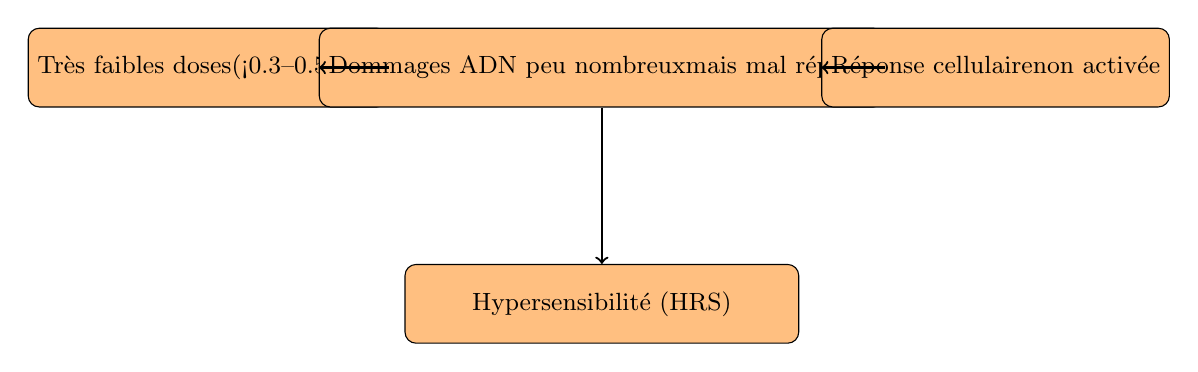
\begin{tikzpicture}[font=\small]

\node[draw, rounded corners, minimum width=4cm, minimum height=1cm, fill=orange!50] (dose) 
    at (0,0) {Très faibles doses\\ (<0.3--0.5 Gy)};

\node[draw, rounded corners, minimum width=4.5cm, minimum height=1cm, fill=orange!50] (dna)
    at (5,0) {Dommages ADN peu nombreux\\ mais mal réparés};

\node[draw, rounded corners, minimum width=4cm, minimum height=1cm, fill=orange!50] (check)
    at (10,0) {Réponse cellulaire\\ non activée};

\node[draw, rounded corners, minimum width=5cm, minimum height=1cm, fill=orange!50] (hrs)
    at (5,-3) {Hypersensibilité (HRS)};

\draw[->, thick] (dose) -- (dna);
\draw[->, thick] (dna) -- (check);
\draw[->, thick] (dna) -- (hrs);

\end{tikzpicture}
\caption{Illustration simplifiée des mécanismes menant à l'hypersensibilité aux très faibles doses.}
\end{figure}
